\subsection{Nach Kaitaia}

Nach Kaitaia


   Fr 21.10.22    Tag 5
  


  Km  101,1 - 115, 6
 


  In den letzten 4 Jahren hat sich die Gegend kaum verändert, das Meer, der Strand, das super Café am Ortsende von Ahipara ,  die hilfsbereiten Menschen, aber leider auch nicht die besch... Wegführung von Ahipara nach Kaitaia und weiter zum Raetea Forest. Es gibt hier zwei Möglichkeiten. Die ungefährliche, sinnvolle, nämlich per Anhalter die nächsten 30 km zurückzulegen, oder die nicht ungefährliche,  sinnbefreite Möglichkeit, das ganze zu Fuß zu erledigen.
 


  (In den Trailnotes des TA wird ausdrücklich die erste Variante empfohlen!)
 


  Nachdem wir die erste Variante vor 4 Jahren schon erprobt hatten und es eigentlich ganz praktisch fanden, entschieden wir uns diese Mal für die zweite Variante...
 


  Nach einem Cappuccino und einem leichten Frühstück im oben genannten Cafe,
 


\begin{figure}[H]
	\centering
	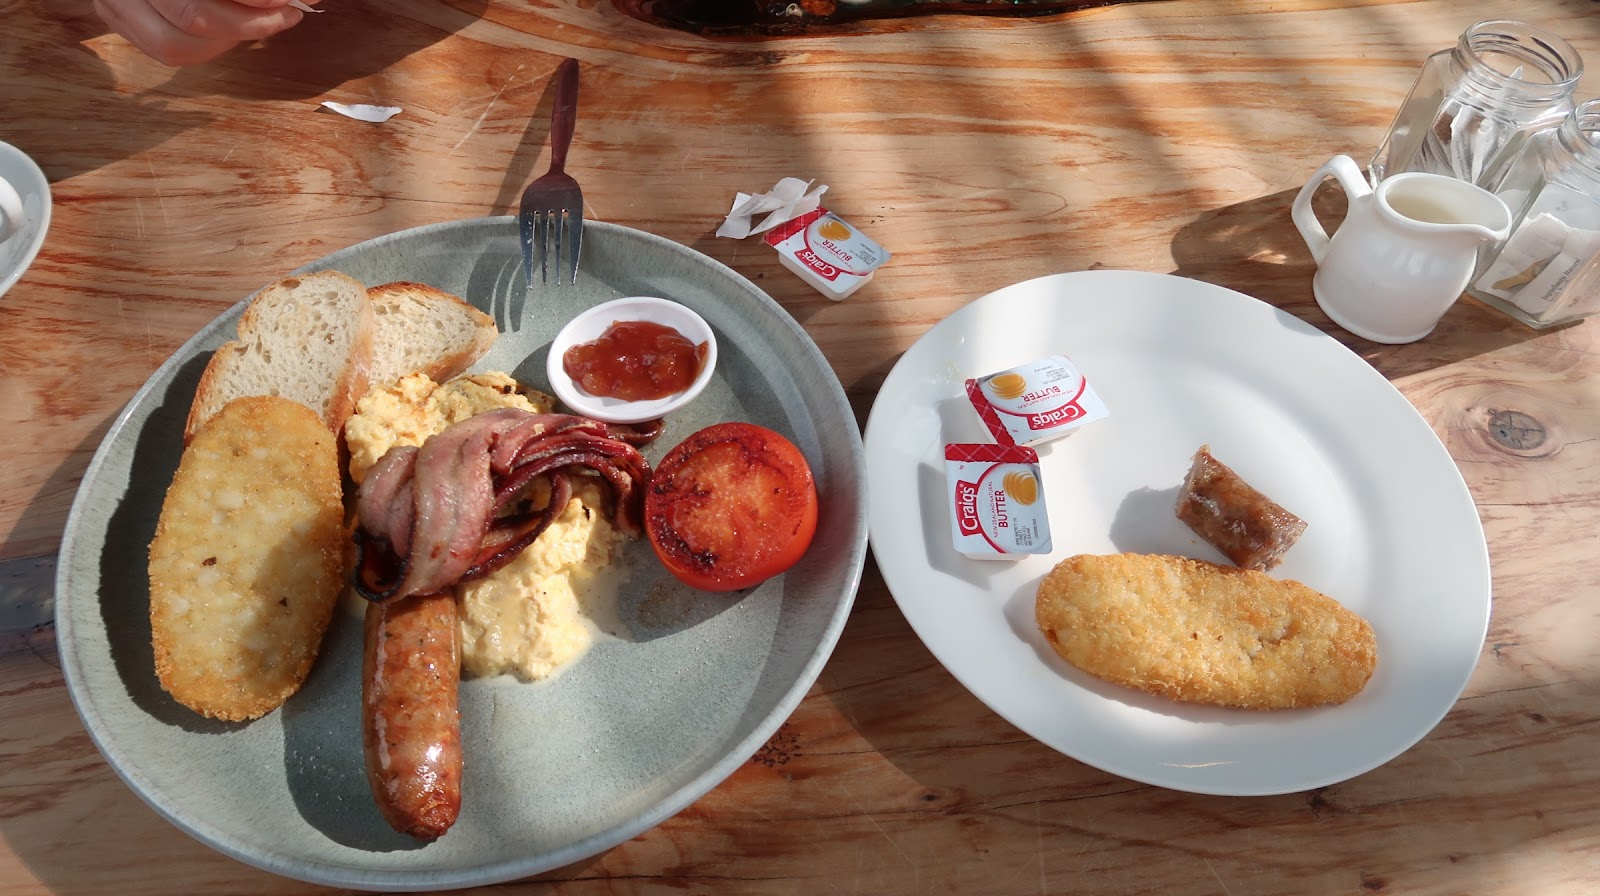
\includegraphics[width=0.5\textwidth]{nach_kaitaia/4_1666344342320822-0.png}
	\caption{}
	\label{fig:4_1666344342320822-0}
\end{figure}

  machen wir uns auf, um drei Stunden und etwa 14 km lang den Verkehr des Highway 1 zu stören. Es gibt hier nicht viele Möglichkeiten  der Straße zu entkommen, meist läuft man direkt am Teerrand, an der Kante eines Entwässerungsgrabens.
 


\begin{figure}[H]
	\centering
	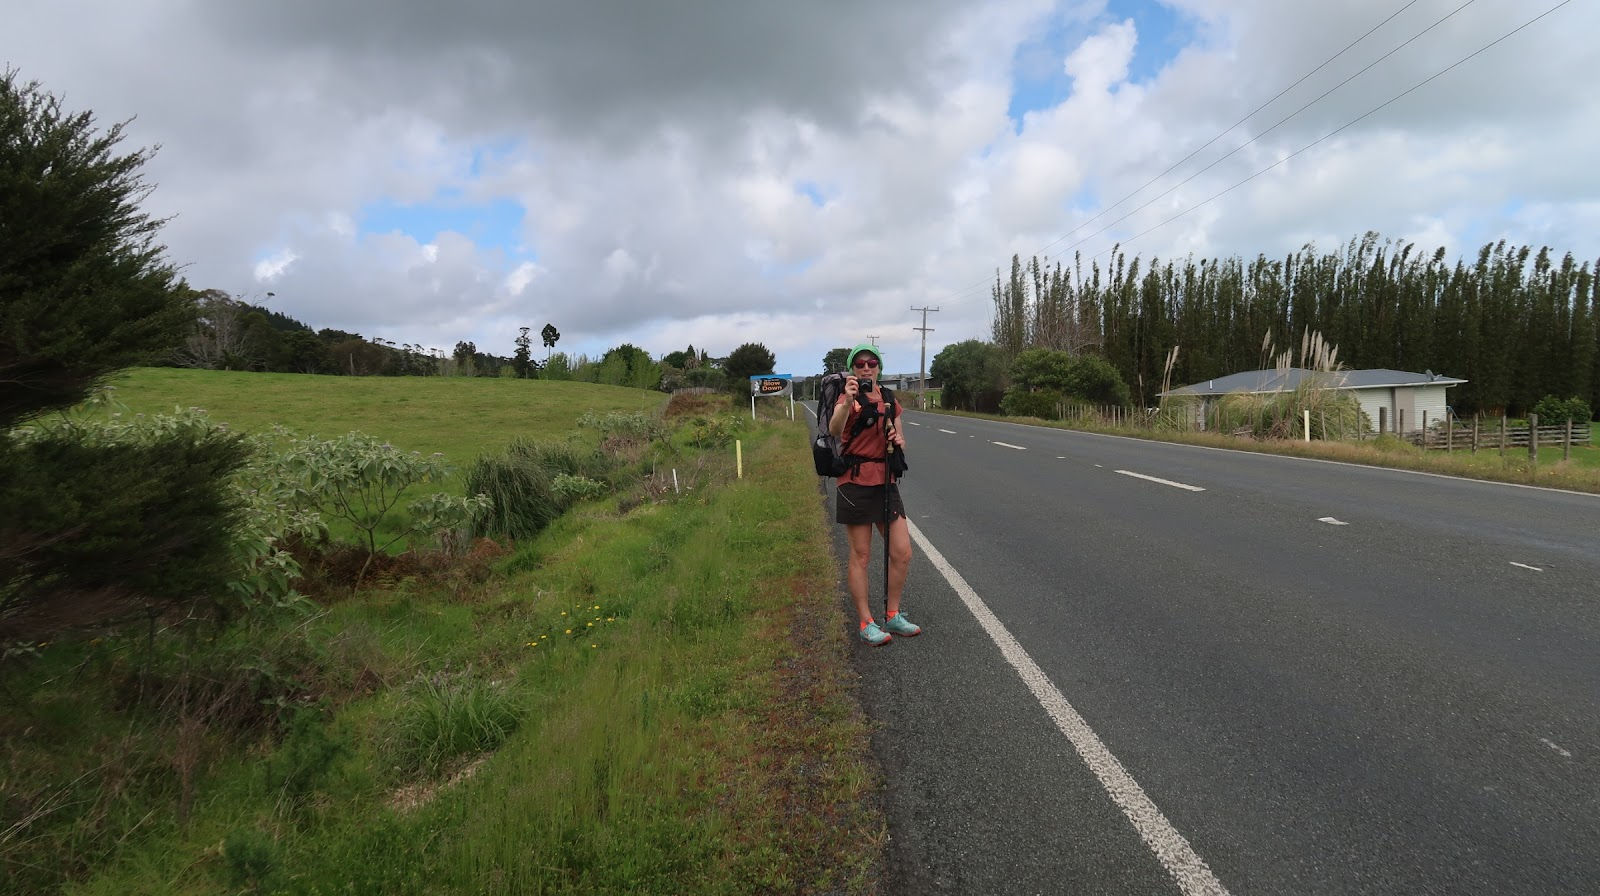
\includegraphics[width=0.5\textwidth]{nach_kaitaia/5_1666344295205985-1.png}
	\caption{}
	\label{fig:5_1666344295205985-1}
\end{figure}

  Wie wir schnell feststellen hat Neuseeland noch immer kein Pfandsystem für Dosen eingeführt und auch die Sache mit den Possums hat sich nicht verändert.
 


\begin{figure}[H]
	\centering
	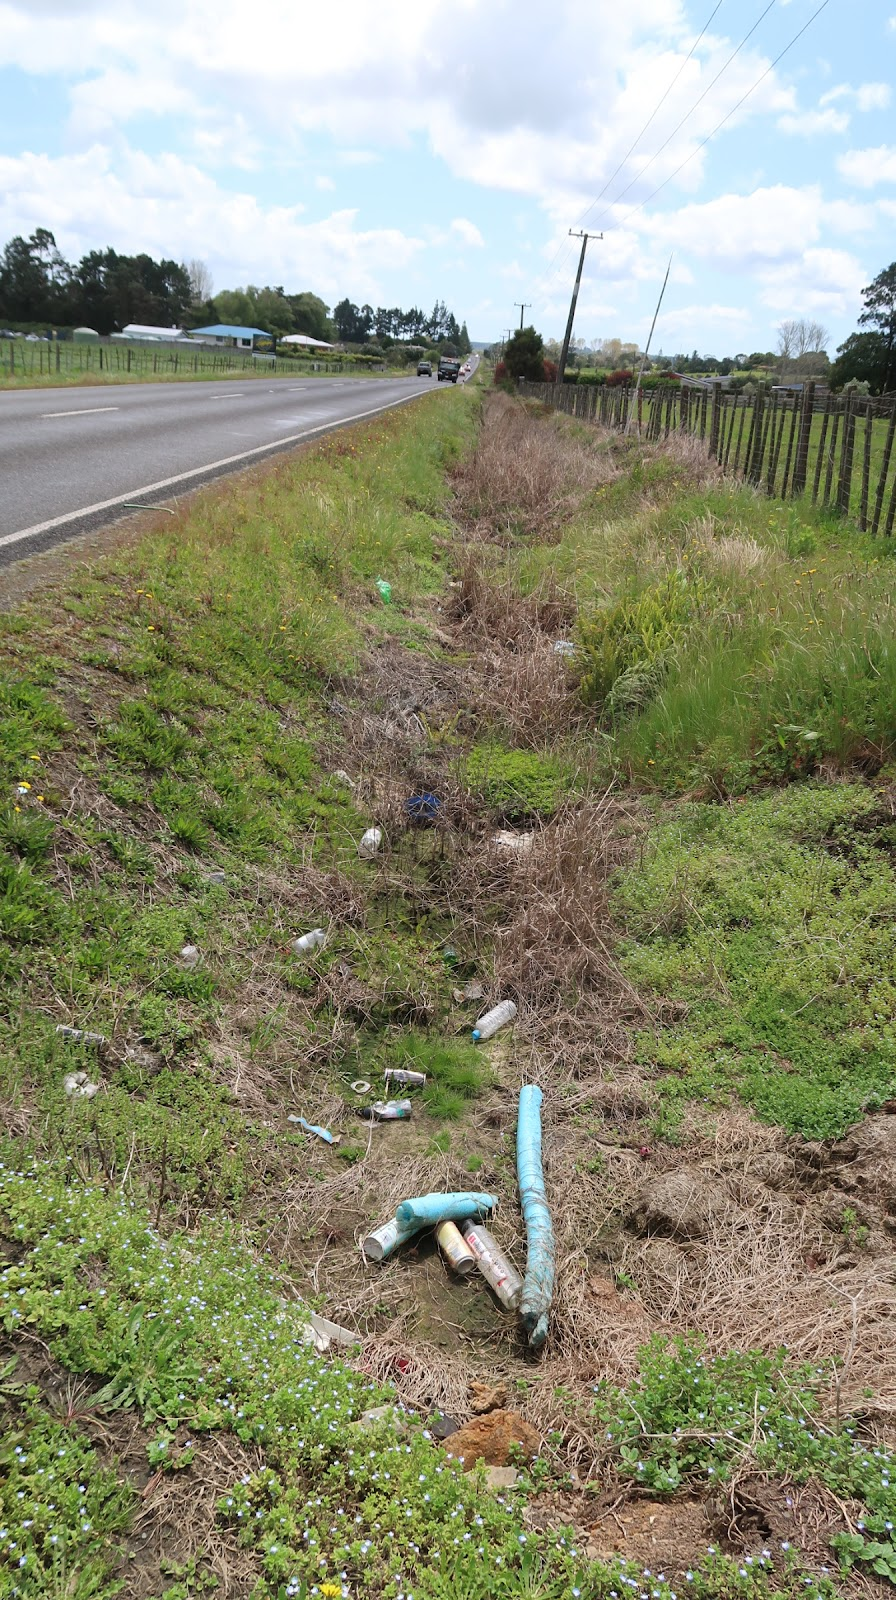
\includegraphics[width=0.5\textwidth]{nach_kaitaia/6_1666344282247967-2.png}
	\caption{}
	\label{fig:6_1666344282247967-2}
\end{figure}

  Auch der Zustand etlicher Häuser an der Straße ließe sich noch verbessern.
 


\begin{figure}[H]
	\centering
	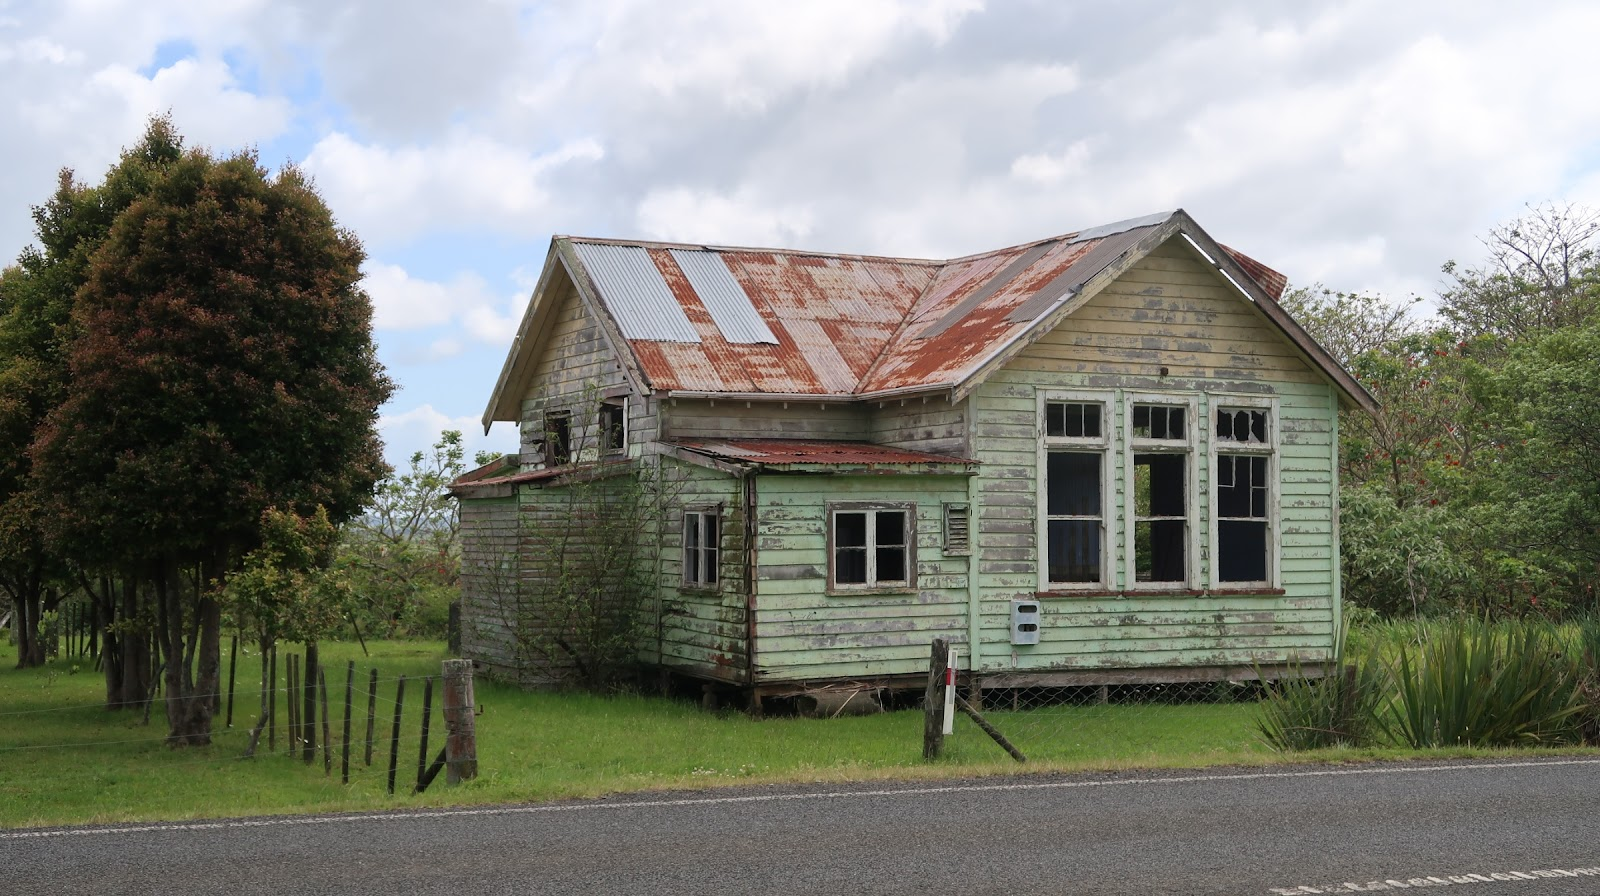
\includegraphics[width=0.5\textwidth]{nach_kaitaia/7_1666344231705325-3.png}
	\caption{}
	\label{fig:7_1666344231705325-3}
\end{figure}

  Das Wetter und unsere Laune ist super, die Beine dagegen eher etwas unmotiviert, aber trotzdem erreichen wir nach knapp 3 Stunden Kaitaia. Schleppen uns in den nächsten Imbiss, Coke, Cappuccino und die ersten richtigen Fish and Chips seit (4!) Jahren.
 


  Ursprünglich hatten wir erwogen nach dem Einkauf der Lebensmittel für die nächsten Tage, noch weiter zu laufen, wir beide sind aber so platt, dass uns schon bald ein nettes Zimmer in einem günstigen Motel willkommen heißt.
 


  gelaufene 15,5 km
 


  Hinweis:
 


  Wir laufen jetzt die nächsten 4-5 Tage durch ein paar Wälder, ohne WLAN und Internet, um dann hoffentlich in Kerikeri wieder aufzutauchen.
 


  Also dann bis bald. ️
 

